\section{Parameter table}\label{app:params}

\begin{table}[H]\centering\footnotesize\renewcommand{\arraystretch}{1.0}\setlength{\tabcolsep}{4pt}
\caption{All model parameters (from \texttt{config/params\_default.yaml}, version 0.3). Where a row lists
several values they are in the order named in the parameter column. ``[verify]'' marks values taken from memory
of public sources that must be checked against the primary document.}\label{tab:params}
\adjustbox{max width=\textwidth}{\begin{tabular}{@{}>{\raggedright\arraybackslash}p{6.9cm}>{\raggedright\arraybackslash}p{4.6cm}>{\raggedright\arraybackslash}p{3.9cm}@{}}
\toprule
Parameter & Value & Source \\
\midrule
\multicolumn{3}{@{}l}{\itshape Issuers} \\
\hangindent=1em\hangafter=0 Supply, A / B, \$bn & 180 / 75 & attestations, 2026 [verify] \\
\hangindent=1em\hangafter=0 Reserves of A: cash / repo / MMF / bills $\leq$1M / bills 1--3M / other & 0.5\% / 10.0\% / 4.0\% / 33.0\% / 33.0\% / 19.5\% & attestation [verify] \\
\hangindent=1em\hangafter=0 Reserves of B: cash / repo / MMF / bills $\leq$1M / bills 1--3M / other & 12.0\% / 48.0\% / 0.0\% / 25.0\% / 15.0\% / 0.0\% & reserve report, look-through [verify] \\
\hangindent=1em\hangafter=0 Other-asset fire-sale haircut & 30\% & assumption \\
\hangindent=1em\hangafter=0 Bill ladder, tb1 / tb3, days & 21 / 42 & assumption \\
\hangindent=1em\hangafter=0 Processing capacity, A / B, \% of supply per day & 1.2\% / 3.0\% & calibrated \\
\hangindent=1em\hangafter=0 Arbitrage capital, A / B, \% of supply per day & 1.1\% / 3.0\% & calibrated \\
\hangindent=1em\hangafter=0 Redemption fee, A / B & 0.1\% / 0.0\% & issuer terms [verify] \\
\hangindent=1em\hangafter=0 Cash hoarding horizon, days & 5 & assumption \\
\addlinespace
\multicolumn{3}{@{}l}{\itshape Treasury-bill market} \\
\hangindent=1em\hangafter=0 Impact anchor flow, \$bn & 3.5 & Ahmed--Aldasoro [verify] \\
\hangindent=1em\hangafter=0 Persistent / temporary sell impact at the anchor, bp per \$bn & 2.0 / 1.0 & Ahmed--Aldasoro outflow range [verify] \\
\hangindent=1em\hangafter=0 Buy impact, bp per \$bn & 0.5 & asymmetry [verify] \\
\hangindent=1em\hangafter=0 Temporary impact decay per day & 0.3 & assumption \\
\hangindent=1em\hangafter=0 Impact shape & square root; linear below the anchor & square-root law \\
\hangindent=1em\hangafter=0 Dealer capacity $K$, \$bn / convexity $\gamma$ / absorption per day & 150 / 2.0 / 0.1 & assumption \\
\hangindent=1em\hangafter=0 MMF reinvestment share $\rho$ / lag, days & 0.5 / 2 & assumption \\
\hangindent=1em\hangafter=0 Duration of bills sold, tb1 / tb3, years & 0.04 / 0.17 & bucket midpoints \\
\addlinespace
\multicolumn{3}{@{}l}{\itshape Holders} \\
\hangindent=1em\hangafter=0 Agents $N$ & 10,000 & design \\
\hangindent=1em\hangafter=0 Type shares of supply: retail / exchange / DeFi / institutional / arbitrageur & 30\% / 30\% / 20\% / 15\% / 5\% & assumption \\
\hangindent=1em\hangafter=0 Attention probability per day, by type & 0.25 / 0.70 / 0.40 / 0.50 / 1.00 & assumption \\
\hangindent=1em\hangafter=0 Exit threshold mean, by type & 0.12 / 0.08 / 0.10 / 0.07 / 0.03 & calibrated (scale 1.0) \\
\hangindent=1em\hangafter=0 Exit threshold s.d., by type & 0.04 / 0.03 / 0.03 / 0.02 / 0.01 & assumption \\
\hangindent=1em\hangafter=0 Signal weights $w_1$, $w_2$, $w_3$, $w_4$ & 0.5, 1.0, 0.3, 0.2 & calibrated / assumption \\
\hangindent=1em\hangafter=0 Private-signal s.d. / common-shock s.d. & 0.02 / 0.005 & assumption \\
\hangindent=1em\hangafter=0 Herding memory / re-entry hysteresis & 0.6 / 0.02 & assumption \\
\hangindent=1em\hangafter=0 Loss probability $\psi$ & 1.0 & calibrated \\
\hangindent=1em\hangafter=0 Belief spillover $\beta$ (E4) & 0, 0.3, 0.6 & assumption \\
\addlinespace
\multicolumn{3}{@{}l}{\itshape Secondary market} \\
\hangindent=1em\hangafter=0 Liquidity depth $\eta$ / arbitrage cost / arbitrage horizon, days & 0.1 / 0.002 / 2 & calibrated / assumption \\
\hangindent=1em\hangafter=0 Suspension discount / price floor & 0.05 / 0.5 & assumption \\
\bottomrule
\end{tabular}
}
\end{table}

\section{Pseudo-code}\label{app:pseudo}

\begin{small}
\begin{enumerate}\setlength{\itemsep}{0pt}
\item Draw the population once per experiment: types, lognormal holdings within type, access flags, attention rates.
\item For each chunk of Monte Carlo paths: initialise reserves from the reserve shares; remove the realised loss from
  other assets, then cash, money market fund shares and repo; draw thresholds $\theta_i$ and private noise
  $\varepsilon_i$; set price $=1$, overhang, queue, herding state and dealer inventory to zero.
\item For each business day $t=1,\dots,30$:
  \begin{enumerate}\setlength{\itemsep}{0pt}
  \item Public expected loss $\ell_t$ (exposure times the loss probability until the resolution day, realised loss
    thereafter); belief $b_t=\ell_t S_0/S_{t-1}$ plus any spillover; signals $x_{it}=b_t+\varepsilon_i$; common
    shock $\nu_t$.
  \item Exit signal~(\ref{eq:signal}); agents who are awake and above threshold exit; exited agents whose core signal
    is below $\theta_i-h$ request re-entry.
  \item Route exits: direct-access holdings to the queue, others to secondary sales $V_t$; update $H_t$.
  \item Arbitrage capacity from daily capital, queue room within $h_a$ days of processing, suspension and the
    fee-plus-cost condition; serve re-entry demand, then arbitrage, from $V_t+O_{t-1}$; set the overhang and
    the price; accepted re-entrants rejoin the population pro rata.
  \item Queue $+=$ direct requests $+$ arbitrage purchases; ladder run-off ($\text{tb1}\to$ cash,
    $\text{tb3}\to\text{tb1}$); demand $=\min(Q_t, cS_0)$ (zero on blackout days); waterfall raises
    demand $\times$ payout (par or net asset value, net of fee); shortfall $\Rightarrow$ suspended; supply and queue fall
    by the tokens paid.
  \item Liquidity management: hoard $=\min(Q_t, h_c\, cS_0)$; reinvest $\min(\text{matured}, \max(0,\text{cash}-\text{hoard}))$
    into $\text{tb1}$; withdrawn $=$ matured $-$ reinvested.
  \item Bill market~(\ref{eq:impact}) with sold, withdrawn and the lagged reinvestment buys $\rho\cdot\text{paid}_{t-L}$;
    fire-sale loss; mark-to-market net asset value; record all series.
  \end{enumerate}
\item Metrics per path (minimum price, redemptions at days 7 and 30, peak impact, bills sold, demand withdrawn,
  suspension days, losses, net asset value) and summaries across paths (medians, 5th and 95th percentiles, run
  probabilities, threshold exceedance probabilities).
\end{enumerate}
\end{small}

\section{Analytic benchmark}\label{app:benchmark}

Consider a continuum of holders of type $k$ with supply shares $\omega_k$, a publicly known loss share $x$ of
reserves that does not change with redemptions, private signals $x_i = x+\varepsilon_i$ with $\varepsilon_i\sim
N(0,\sigma^2)$ and exit cutoffs $\theta_i\sim N(\bar\theta_k,\tau_k^2)$. In the limit without herding, depeg and
suspension channels, holder $i$ exits within the horizon if $x+\varepsilon_i>\theta_i$, so the share of supply that
exits is
\begin{equation}
E(x) \;=\; \sum_k \omega_k\, \Phi\!\left(\frac{x-\bar\theta_k}{\sqrt{\sigma^2+\tau_k^2}}\right).
\end{equation}
In a global game with a fire-sale liquidation cost $c(n)$ increasing in the exiting mass $n$, as in
\citet{goldstein2005} and \citet{morris2016}, the equilibrium cutoff $\theta^*$ falls as the liquidation cost
rises, $\partial\theta^*/\partial c<0$: a costlier fire sale makes the run start at a smaller loss. In our model the
fire-sale cost on bills is tiny because bill duration is tiny, so this amplification is absent and the cutoffs are
calibrated rather than derived. Table~\ref{tab:benchmark} and Figure~\ref{fig:f6} compare the simulated exit share
with $E(x)$ when $w_1=w_3=w_4=0$, $\sigma_\nu=0$ and the belief is held fixed: the two agree to within a tenth of a
percentage point.

\begin{table}[H]\centering\small
\caption{Benchmark check: share of supply exiting within 30 days in the simulation with the behavioural channels
off (100 paths) against the closed-form threshold aggregate.}
\label{tab:benchmark}
\begin{tabular}{rrr}
\toprule
Loss share & ABM exit share & Closed form \\
\midrule
0\% & 1.0\% & 1.1\% \\
2\% & 4.2\% & 4.3\% \\
4\% & 11.6\% & 11.6\% \\
6\% & 24.0\% & 24.0\% \\
8\% & 40.8\% & 40.9\% \\
10\% & 59.0\% & 59.0\% \\
12\% & 74.6\% & 74.6\% \\
15\% & 89.9\% & 90.0\% \\
20\% & 98.9\% & 98.8\% \\
\bottomrule
\end{tabular}

\end{table}

\begin{figure}[H]\centering
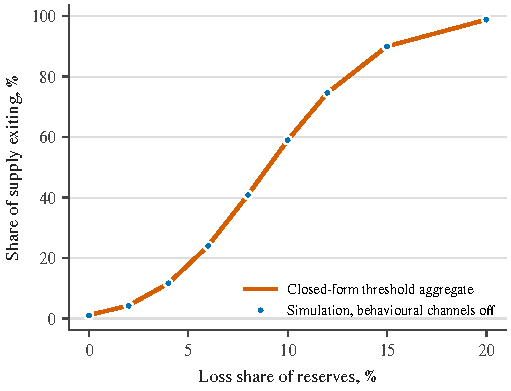
\includegraphics[width=0.55\textwidth]{F6_benchmark_check}
\caption{Benchmark check: simulated exit share with the behavioural channels off against the closed-form threshold
aggregate.}\label{fig:f6}
\end{figure}

\section{Additional results}\label{app:extra}

\begin{table}[H]\centering\small
\caption{E1 baseline for Issuer~B (1{,}000 paths). Same scenarios as Table~\ref{tab:e1}; Issuer~B has no cushion of
other assets, so a realised loss hits deposits and the reserve fund directly, and its processing capacity is 3\% of
supply per day.}\label{tab:e1B}
\adjustbox{max width=\textwidth}{\begin{tabular}{lrrrrr}
\toprule
Metric & No shock & 5\% loss & 10\% loss & 20\% loss & 8\% exposure, resolved \\
\midrule
Minimum token price (median) & 0.998 & 0.607 & 0.500 & 0.500 & 0.904 \\
Redeemed by day 7 & 1.9\% & 21.0\% & 21.0\% & 21.0\% & 18.0\% \\
Redeemed by day 30 & 2.3\% & 90.0\% & 90.0\% & 80.0\% & 24.0\% \\
P(redemptions $\geq$ 20\%) & 0\% & 100\% & 100\% & 100\% & 99\% \\
P(redemptions $\geq$ 50\%) & 0\% & 100\% & 100\% & 100\% & 0\% \\
Peak 3M bill-yield impact, bp (median) & 0.0 & 0.6 & 8.6 & 12.6 & 1.8 \\
Peak impact, bp (95th pct.) & 0.0 & 0.6 & 8.6 & 12.6 & 1.8 \\
Bills sold outright, \$bn & 0.0 & 0.4 & 4.3 & 7.7 & 0.0 \\
Maturing bills not rolled, \$bn & 0.0 & 25.9 & 25.7 & 22.3 & 7.1 \\
Peak net bill demand withdrawn, \$bn & 0.0 & 0.1 & 2.5 & 4.7 & 0.9 \\
Other assets sold, \$bn & 0.0 & 0.0 & 0.0 & 0.0 & 0.0 \\
P(any suspension day) & 0\% & 0\% & 100\% & 100\% & 0\% \\
Fire-sale and haircut loss, \$bn & 0.00 & 0.00 & 0.00 & 0.00 & 0.00 \\
NAV on day 30 (median) & 1.000 & 0.500 & 0.000 & 0.000 & 1.000 \\
\bottomrule
\end{tabular}
}
\end{table}

\begin{figure}[H]\centering
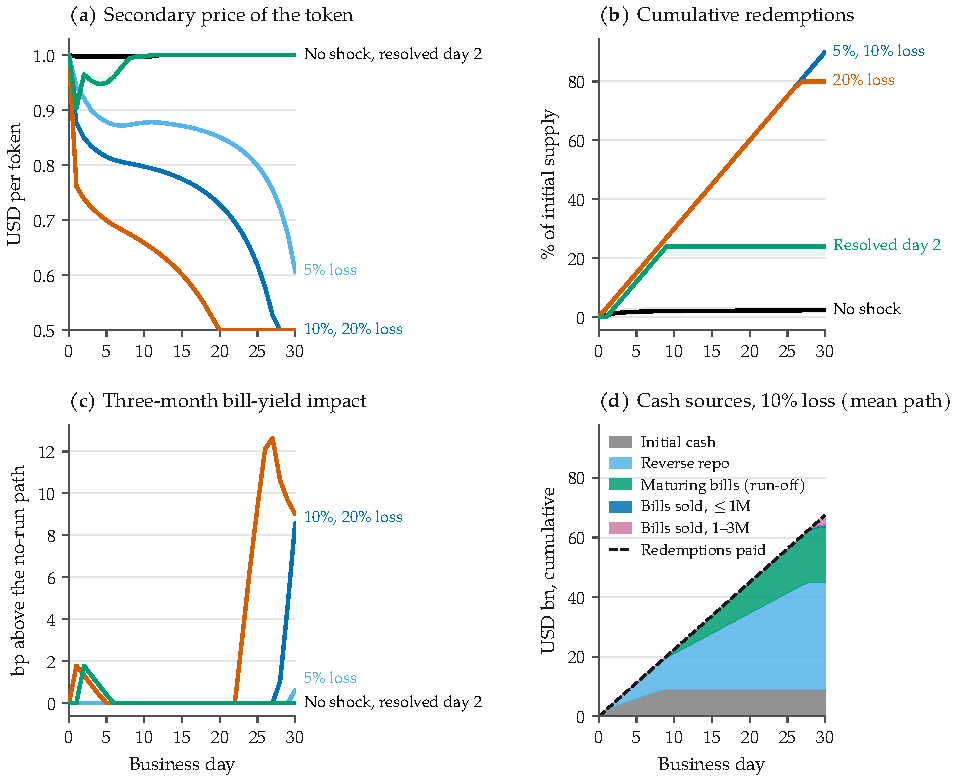
\includegraphics[width=\textwidth]{F1_B_baseline_dynamics}
\caption{Baseline run dynamics for Issuer~B (1{,}000 paths), panels as in Figure~\ref{fig:f1}.}\label{fig:f1b}
\end{figure}
